\setAuthor{Valter Kiisk}
\setRound{lahtine}
\setYear{2023}
\setNumber{G 8}
\setDifficulty{8}
\setTopic{TODO}

\prob{Lääts}
\begin{wrapfigure}[8]{r}{0.2\linewidth}
    \vspace{-30pt}
    \begin{center}
        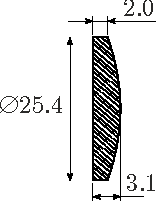
\includegraphics[width=\linewidth]{2023-lahg-08-yl.pdf}
    \end{center}
\end{wrapfigure}
Joonisel on kujutatud teatava tasakumera läätse ristlõige ja selle mõõdud millimeetrites. Lääts on valmistatud klaasist, mille murdumisnäitaja $n=\num{1.52}$.\\
\osa Eeldusel, et kumerpind on sfääriline, kui suur on selle kõverusraadius?\\
\osa Määrake läätse fookuskaugus kiirte jaoks, mis kulgevad optilise peatelje lähedal (Võite eeldada, et lääts on õhuke, st piisab 3 mm täpsusega õigest vastusest.)! \\ \emph{Märkus:} Väikeste nurkade $x$ korral võib kasutada lähendust $\sin{x} \approx \tan{x} \approx x$ (nurk $x$ on radiaanides).



\hint

\solu
\osa Tähistame läätse raadiuse $r=\frac{1}{2}\cdot \SI{25.4}{mm}=\SI{12.7}{mm}$ (vt joonis). Läätse kumerpinnaga kaetud osa paksus on ilmselt $h = \SI{3.1}{mm} - \SI{2.0}{mm} = \SI{1.1}{mm}$. Nüüd Pythagorase teoreemi põhjal $R^2 = r^2 + (R - h)^2$, millest
\[
R = \frac{r^2 + h^2}{2h} = \frac{(\SI{12.7}{mm})^2 + (\SI{1.1}{mm})^2}{2\cdot \SI{1.1}{mm}}\approx \SI{73.8}{mm}.
\]

\osa Läätsele langevad paralleelsed kiired koonduvad fookuses. Õhukese läätse eeldusel võime fookuskauguseks lugeda lihtsalt fookuspunkti kauguse mistahes murdvast pinnast. Kõige lihtsam on seda analüüsi teha valguskiire jaoks, mis langeb läätsele vasakult, paralleelselt optilise peateljega. Seega esimesel pinnal murdumist ei toimu. Olgu langemisnurk kumerpinnale $\alpha$ ja murdumisnurk $\gamma$. Snelli seadusest $n\sin\alpha=\sin\gamma$. Kuna valguskiir eeldatavasti kulgeb optilise peatelje lähedal, siis kõik nurgad on väikesed, nii et $\sin\alpha\approx\alpha$ ja $\sin\gamma\approx\gamma$. Seega $\gamma\approx n\alpha$ ja $\varphi=\gamma-\alpha\approx(n-1)\alpha$. Langev kiir kulgeb optilisest teljest kaugusel $a=R\sin\alpha\approx \alpha R$. Samamoodi, pärast murdumist $\varphi f\approx a$ ehk
\[
f\approx\frac{a}{\varphi}=\frac{\alpha R}{(n-1)\alpha}=\frac{R}{n-1}\approx \SI{142}{mm}.
\]

\begin{center}
  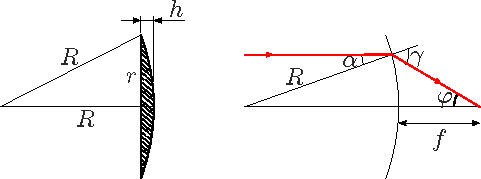
\includegraphics{2023-lahg-08-sol.pdf}
\end{center}
\probend